% Created 2023-08-31 Thu 12:32
% Intended LaTeX compiler: pdflatex

% =================================BASE====================================%
\documentclass[10pt]{article}
\usepackage[left=2cm,right=2cm,top=2cm,bottom=2cm]{geometry} % Marges
%\usepackage{libertine}
%\usepackage{libertinust1math}
\usepackage[T1]{fontenc} % Nécessaire avec FrenchBabel
\usepackage[utf8]{inputenc} % Important pour symboles Francophones, é,à,etc

\usepackage{lmodern}
\renewcommand{\familydefault}{cmr} % La meilleure police (CMU Serif Roman) (Je me suis battu).
\usepackage{mathrsfs} %Permet la command \mathscr (Lettres attachées genre)

\usepackage{natbib} % Bibliographie
\bibliographystyle{abbrvnat}



\usepackage{amsmath, amssymb, amsthm} % Symb. math. (Mathmode+Textmode) + Beaux théorèmes.

\usepackage{mathtools,cancel} % Utilisation de boîtes \boxed{} + \cancelto{}{}
\usepackage{graphicx, wrapfig} % Géstion des figures.
\usepackage{hyperref} % Permettre l'utilisation d'hyperliens.
\usepackage{color} % Permettre l'utilisation des couleurs.
\usepackage[dvipsnames]{xcolor} % Couleurs avancées.
\usepackage{titling} % Donne accès à \theauthor, \thetitle, \thedate

% >>> Physique >>>
\usepackage{physics} % Meilleur package pour physicien. 
\usepackage{pxfonts} % Rajoute PLEIN de symboles mathématiques, dont les intégrales doubles et triples
% <<< Physique <<<

\usepackage{lipsum} % For fun
\usepackage{tikz} % Realisation de figures TIKZ.
\usepackage{empheq} % Boite autour de MULTIPLE équations

\usepackage[french]{babel} % Environnements en Français.
% ==============================BASE-(END)=================================%



% ================================SETTINGS=================================%
% Pas d'indentation en début de paragraphe :
\setlength\parindent{0pt} 

% Couleurs de hyperliens :
\definecolor{mypink}{RGB}{147, 0, 255}
\hypersetup{colorlinks, urlcolor=mypink, citecolor=mypink, linkcolor=mypink}

% Numéros d'équations suivent les sections :
\numberwithin{equation}{section} 

% Les « captions » sont en italique et largeur limitée
\usepackage[textfont = it]{caption} 
\captionsetup[wrapfigure]{margin=0.5cm}

% Retirer le l'écriture en gras dans la table des matières
\usepackage{tocloft}
\renewcommand{\cftsecfont}{\normalfont}
\renewcommand{\cftsecpagefont}{\normalfont}

% Change bullet style
\usepackage{pifont}
\usepackage{enumitem}
%\setlist[itemize,1]{label=\ding{224}}
\setlist[itemize,1]{label=\ding{239}}
\renewcommand{\boxtimes}{\blacksquare}
% ================================SETTINGS=================================%



% ==============================NEWCOMMANDS================================%
% Degrés Celsius :
\newcommand{\celsius}{${}^\circ$ C} % \degrée Celsius : Pas mal plus simple qu'utilise le package gensymb qui plante avec tout...

% Vecteurs de base :
\newcommand{\nvf}{\vb{\hat{n}}}
\newcommand{\ivf}{\vb{\hat{i}}}
\newcommand{\jvf}{\vb{\hat{j}}}
\newcommand{\kvf}{\vb{\hat{k}}}

\newcommand{\uu}{\vb*{u}}
\newcommand{\vv}{\vb*{v}}

% Boîte vide pour ajuster les underbrace
\newcommand{\bigno}{\vphantom{\qty(\frac{d}{q})}}
\newcommand{\pt}{\hspace{1pt}}

% Physics empty spaces 
\newcommand{\typical}{\vphantom{A}}
\newcommand{\tall}{\vphantom{A^{x^x}_p}}
\newcommand{\grande}{\vphantom{\frac{1}{xx}}}
\newcommand{\venti}{\vphantom{\sum_x^x}}

% Moyenne numérique entre deux points de grilles. 
\newcommand{\xmean}[1]{\overline{#1}^x}
\newcommand{\ymean}[1]{\overline{#1}^y}
\newcommand{\zmean}[1]{\overline{#1}^z}
\newcommand{\xymean}[1]{\overline{#1}^{xy}}

% Tilde over psi
\newcommand{\tpsi}{\tilde{\psi}}
\newcommand{\tphi}{\tilde{\phi}}

% Nota Bene env :
\newcommand{\nb}{\ding{165}\ \textbf{N.B.}\hspace{4pt}}
   
% ==============================NEWCOMMANDS================================%



% ==============================PAGE-TITRE=================================%
% Titlepage 
\newcommand{\mytitlepage}{
\begin{titlepage}
\begin{center}
{\Large Contrat Été 2023 \par}
\vspace{2cm}
{\Large \MakeUppercase{\thetitle} \par}
\vspace{2cm}
RÉALISÉ DANS LE CADRE\\ D'UN PROJET POUR \par
\vspace{2cm}
{\Large ISMER--UQAR \par}
\vspace{2cm}
{\thedate}
\end{center}
\vfill
Rédaction \\
{\theauthor}\\
\url{charles-edouard.lizotte@uqar.ca}\\
ISMER-UQAR
\end{titlepage}
}
% ==============================PAGE-TITRE=================================%



% =================================ENTÊTE==================================%
\usepackage{fancyhdr}
\pagestyle{fancy}
\setlength{\headheight}{13pt}
\renewcommand{\headrulewidth}{1.3pt} % Ligne horizontale en haut

\fancyhead[R]{\textit{\thetitle}}
\fancyhead[L]{\ \thepage}
\fancyfoot[R]{\textit{\theauthor}}
\fancyfoot[L]{}
\fancyfoot[C]{} 
% =================================ENTÊTE==================================%
\author{Charles-Édouard Lizotte}
\date{01/09/2023}
\title{Carnet de bord, Université McGill}
\hypersetup{
 pdfauthor={Charles-Édouard Lizotte},
 pdftitle={Carnet de bord, Université McGill},
 pdfkeywords={},
 pdfsubject={},
 pdfcreator={Emacs 27.1 (Org mode 9.6.7)}, 
 pdflang={French}}
\begin{document}

\mytitlepage
\tableofcontents\newpage

\section{Diatribes mathématiques -- \textit{<2023-08-28 Mon>}}
\label{sec:org91e80ff}
L'implémentation de MUDPACK et notre insatisfaction m'amène à voir s'il y aurait d'autres méthodes mathématiques pour résoudre notre problème.
En somme, l'équation différentielle partielle à résoudre est une équation elliptique -- plus précisément une équation de Poisson -- composée d'une dérivée de second ordre et d'une autre de premier ordre.
Soit,
\begin{equation}
\label{eq:org02fb980}
   \laplacian{\psi} = \kvf \cdot \curl{\uu_{BT}}.
\end{equation}
L'équation \ref{eq:org02fb980} est composée de dérivées de second ordre, mais existe-t-il un moyen de la réduire au premier ordre, considérant que l'erreur induite dans \emph{MUDPACK} est affectée par la précision des chiffres significatifs?
La réponse est probablement négative, mais essayons quand même pour se redonner confiance.
Utilisons la relation
\begin{equation}
   \curl(\vb{A}\times\vb{B}) = \vb{A}\qty(\divergence{\vb{B}}) - \vb{B}\qty(\divergence{\vb{A}}) +\qty(\vb{B}\cdot\gradient)\vb{A} -\qty(\vb{A}\cdot\gradient)\vb{B}.
\end{equation}
En premier, comme le courant est donné par la relation \(\uu_{BT} = \kvf \times \gradient{\psi}\), on peut développer l'équation \ref{eq:org02fb980},
\begin{align}
   \div{\gradient{\psi}}
   \venti&= \kvf \cdot \qty(\kvf \times \gradient{\psi}),\nonumber \\
   \venti&= \kvf \cdot \big(\kvf\qty(\divergence{\gradient{\psi}}) - \cancelto{0}{\gradient{\psi}\qty(\divergence{\kvf})} + \qty(\kvf\cdot\gradient) \gradient{\psi} - \cancelto{0}{\qty(\gradient{\psi} \cdot\gradient)\kvf} \big),\nonumber\\
   \venti&= \kvf \cdot \qty(\kvf\qty(\divergence{\gradient{\psi}}) + \qty(\kvf\cdot\gradient) \gradient{\psi}),\nonumber\\
   \venti&= \divergence{\gradient{\psi}} + \cancelto{0}{(\kvf\cdot\gradient)\gradient(\psi)},\nonumber\\
   \venti&=\divergence{\gradient{\psi}}.
\end{align}
Ouin\ldots{} dommage. Les maths fonctionnent en tout cas\ldots{}

\section{Fishpack -- \textit{<2023-08-29 Tue>}}
\label{sec:org811059c}

\begin{figure}[!htpb]
\centering
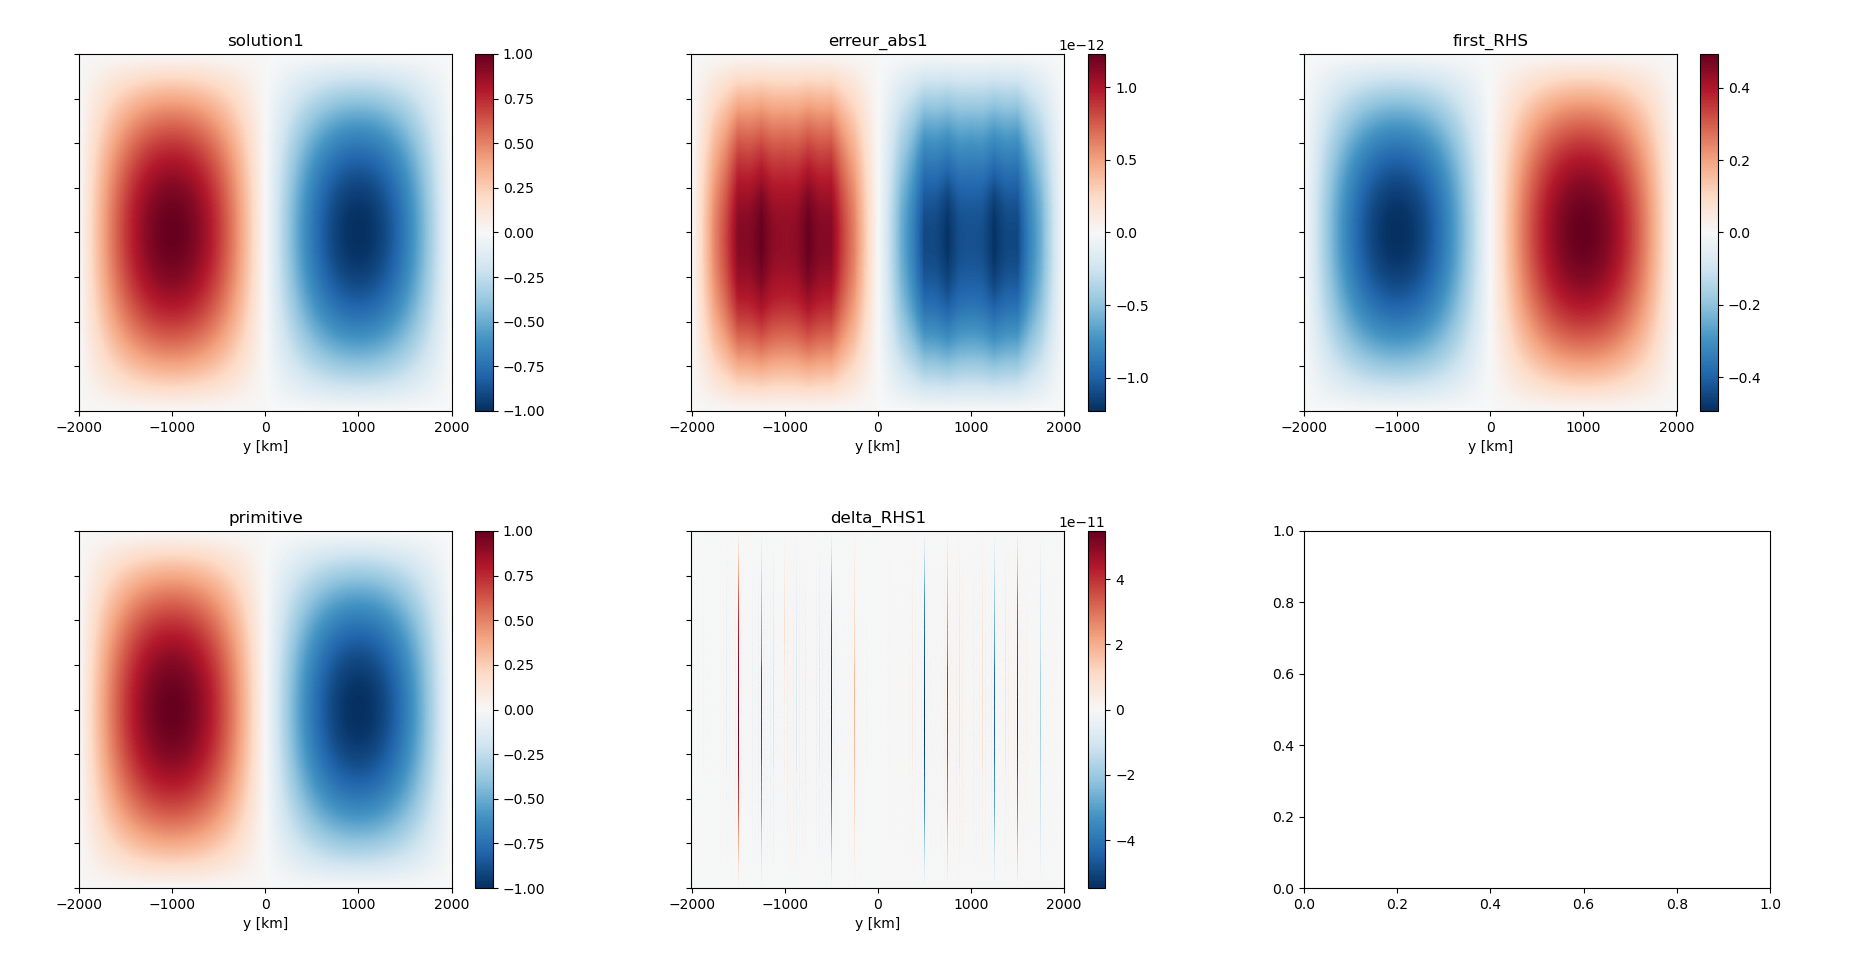
\includegraphics[width=0.8\textwidth]{figures/fishpack/2023-08-29-fishtest.png}
\caption{\label{fig:org536b02b}Comparaison des mêmes quantités évaluées avec MUDPACK, mais avec le solveur Fishpack. Résultat ahurissant.}
\end{figure}

Ce lundi soir et mardi, j'étais un peu épuisé qu'on perde autant de temps sur \emph{MUDPACK}, c'est pourquoi j'ai commencé à regarder ailleurs.
Entre autre, un article en ligne comparait l'efficacité de trois méthodes pour solutionner rapidement les équations différentielles partielles du genre de celle à laquelle on a affaire (équation \ref{eq:org02fb980}).\bigskip

Concrétement, \emph{MUDPACK} était la moins bonne, mais il mentionnait un autre module nommé \emph{fishpack}.
Donc, je me suis lancé.
Deux versions existaient en ligne, soit celle de NCAR et une \href{https://github.com/jlokimlin/fishpack}{version mise à jour} il y a 6 ans.
Bien entendu j'ai pris la plus récente pour m'assurer qu'on puisse utiliser les type DOUBLE PRECISION.\bigskip

Après une journée de travail, j'en suis arrivé à la figure \ref{fig:org536b02b}.
Le résultat est ahurissant, on obtient une erreur absolue de l'ordre de \(10^{-12}\) et un écart de \(\zeta\) de \(10^{-11}\).
On peut en déduire de \emph{MUDPACK} est complétement surclassé.
Sans oublier que le temps de calcul est minimal aussi.

\subsection{Implémentation dans le modèle en eau peu profonde -- \textit{<2023-08-30 Wed>}}
\label{sec:orgb9e8ff1}

Comme au premier jet, nous solvons l'équation \ref{eq:org02fb980} directement.
Donc, aucun besoin de corriger le RHS ou l'écart entre les deux champs : on corrige directement le champ courant (donc celui mis à jour : \(ilevel=3\)).
Si le besoin pour une meilleure précision se fait sentir, on pourra revenir à nos bonnes habitudes de seulement corriger l'écart entre les champs \(ilevel=1\) et \(ilevel=3\), de sorte à suivre le pas de temps de type \emph{leapfrog}.

\subsubsection{Rappel de l'analyse dimensionelle associée au vent \textit{<2023-08-31 Thu>}}
\label{sec:org25a2467}
La nuit dernière, j'ai lancé une simulation de 10 ans, mais nous sommes toujours dans le \emph{spin up}.
Après un peu de bébroussaillage, j'ai vu que ça venait probablement du \(\tau\) insuffisant.,
À la base, j'avais mis ça car David voulait voir le système évoluer sans les termes non-linéaires et je l'avais oublié là.
J'ai relancé la simulation avec un vent de \(\tau = 0.1 Nm^{-2}\).\bigskip

Les paramètres sont illustrés dans le tableau \ref{tab:org631b0dc}.

\begin{table}[htbp]
\caption{\label{tab:org631b0dc}Paramètres utilisés dans la simulation de jeudi matin (\textit{<2023-08-31 Thu>}).}
\centering
\begin{tabular}{llrl}
\hline
\hline
Paramètres & Symbole & Valeur & Unité\\[0pt]
\hline
Taille du domaine & L\textsubscript{x} = L\textsubscript{y} & 2000 & km\\[0pt]
Nombre de points de grilles & nx = ny & 513 & --\\[0pt]
Pas de temps & \(\Delta\) t & 300 & s\\[0pt]
Paramètre de Coriolis & f & 7\texttimes{}10\textsuperscript{-5} & s\textsuperscript{-1}\\[0pt]
Paramètre beta & beta & 1\texttimes{}10\textsuperscript{-11} & m\textsuperscript{-1}s\textsuperscript{-1}\\[0pt]
Amplitude du vent & \(\tau\)\textsubscript{atm} & 0.1 & N m\textsuperscript{-2}\\[0pt]
Coefficient de visc. biharmonique & A\textsubscript{bh} & dx\textsuperscript{4} \texttimes{}10\textsuperscript{-5} & s\textsuperscript{-1}\\[0pt]
Coefficient de frottement & r\textsubscript{drag} & 10\textsuperscript{-7} & s\textsuperscript{-1}\\[0pt]
Vitesse des ondes internes barocliniques & c\textsubscript{bc} & 2 & ms\textsuperscript{-1}\\[0pt]
Épaisseur de la couche supérieure & H\textsubscript{1} & 1000 & m\\[0pt]
Épaisseur de la couche inférieur & H\textsubscript{2} & 3000 & m\\[0pt]
\hline
\end{tabular}
\end{table}

L'analyse dimensionnel va comme suit : Pour l'évolution,
\begin{equation}
   \pdv{\uu}{t} \Rightarrow \qty[ \frac{ms^{-1}}{s}] \Rightarrow \qty[\frac{m}{s^2}]. 
\end{equation}

Pour le terme associé au frottement visqueux du vent à la surface,
\begin{equation}
   \frac{\tau}{\rho h} \Rightarrow \frac{\qty[N m^{-2}]}{\qty[Kg\cdot m^{-3}] \qty[m]} \Rightarrow \qty[\frac{N}{Kg}] \Rightarrow \frac{\qty[Kg \cdot m s^{-2}]}{[Kg]} \Rightarrow \qty[\frac{m}{s^2}].
\end{equation}
Bonne nouvelle! Notre schéma pour le frottement visqueux à la surface est bon et je ne fais pas des erreurs stupides depuis 6 mois! \emph{Cheers!}
\end{document}